% Crear pdf con:
% pdflatex -synctex=1 -interaction=nonstopmode %.tex
%"The PDF file may contain up to 25 pages of reference material, single-sided, letter or A4 size, with text and illustrations readable by a person with correctable eyesight without magnification from a distance of 1/2 meter."
%%% hidelinks quita los recuadros rojos de los links.
\documentclass[10pt,landscape,twocolumn,a4paper,notitlepage, hidelinks]{article} 
\usepackage{hyperref}
\usepackage[spanish, activeacute]{babel}
\usepackage[utf8]{inputenc}
\usepackage{fancyhdr}
\usepackage{lastpage}
\usepackage{listings}
\usepackage{amssymb}
\usepackage[usenames,dvipsnames]{color}
\usepackage{graphicx}
\usepackage{wrapfig}
\usepackage{amsmath}
\usepackage{makeidx}

%%% Margenes
\setlength{\columnsep}{0.25in}    % default=10pt
\setlength{\columnseprule}{0.5pt}    % default=0pt (no line)
 
\addtolength{\textheight}{2.35in}
\addtolength{\topmargin}{-0.9in}     % ~ -0.5 del incremento anterior
 
\addtolength{\textwidth}{1.1in}
\addtolength{\oddsidemargin}{-0.55in} % -0.5 del incremento anterior
 
\setlength{\headsep}{0.08in}
\setlength{\parskip}{0in}
\setlength{\headheight}{15pt}
\setlength{\parindent}{0mm}
 
%%% Encabezado y pie de pagina
\pagestyle{fancy}
\fancyhead[LO]{\textbf{\title}}
\fancyhead[C]{\leftmark\ -\ \rightmark}
\fancyhead[RO]{P\'agina \thepage\ de \pageref{LastPage}}
\renewcommand{\headrulewidth}{0.4pt}
\fancyfoot{}
\definecolor{darkblue}{rgb}{0,0,0.4}
%%% Configuracion de Listings
\lstloadlanguages{C++}
\lstnewenvironment{code}
	{%\lstset{	numbers=none, frame=lines, basicstyle=\small\ttfamily, }%
	 \csname lst@SetFirstLabel\endcsname}
	{\csname lst@SaveFirstLabel\endcsname}
\lstset{% general command to set parameter(s)
	language=C++, basicstyle=\small\ttfamily, keywordstyle=\slshape,
	emph=[1]{usa}, emphstyle={[1]\sffamily\bfseries},
	morekeywords={tint,forn,forsn,node,alt,tipo},
	basewidth={0.47em,0.40em},
	columns=fixed, fontadjust, resetmargins, xrightmargin=5pt, xleftmargin=15pt,
	flexiblecolumns=false, tabsize=2, breaklines,	breakatwhitespace=false, extendedchars=true,
	numbers=left, numberstyle=\tiny, stepnumber=1, numbersep=9pt,
	frame=l, framesep=3pt,
    basicstyle=\ttfamily,
    keywordstyle=\color{darkblue}\ttfamily,
    stringstyle=\color{magenta}\ttfamily,
    commentstyle=\color{RedOrange}\ttfamily,
    morecomment=[l][\color{OliveGreen}]{\#}
}

\lstdefinestyle{C++}{
	language=C++, basicstyle=\small\ttfamily, keywordstyle=\slshape,
	emph=[1]{usa,tipo2}, emphstyle={[1]\sffamily\bfseries},
	morekeywords={tint,forn,forsn,tipo,alt,node},
	basewidth={0.47em,0.40em},
	columns=fixed, fontadjust, resetmargins, xrightmargin=5pt, xleftmargin=15pt,
	flexiblecolumns=false, tabsize=2, breaklines,	breakatwhitespace=false, extendedchars=true,
	numbers=left, numberstyle=\tiny, stepnumber=1, numbersep=9pt,
	frame=l, framesep=3pt,
    basicstyle=\ttfamily,
    keywordstyle=\color{darkblue}\ttfamily,
    stringstyle=\color{magenta}\ttfamily,
    commentstyle=\color{RedOrange}\ttfamily,
    morecomment=[l][\color{OliveGreen}]{\#}
}
 
%%% Macros
\def\nbtitle#1{\begin{Large}\begin{center}\textbf{#1}\end{center}\end{Large}}
\def\nbsection#1{\section{#1}}
\def\nbsubsection#1{\subsection{#1}}
\def\nbcoment#1{\begin{small}\textbf{#1}\end{small}}
\newcommand{\comb}[2]{\left( \begin{array}{c} #1 \\ #2 \end{array}\right)}
\def\complexity#1{\texorpdfstring{$\mathcal{O}(#1)$}{O(#1)}}
 \newcommand\cppfile[2][]{
\lstinputlisting[style=C++,linerange={#1}]{#2}
}

%%% Configuración de paths

\makeatletter
\def\input@path{{../}}
\makeatother

%%% Arregla espacios

\frenchspacing

\begin{document}
\def\title{El Mastro - Mastropiero Limit Exceeded - UNS}

\begin{center}{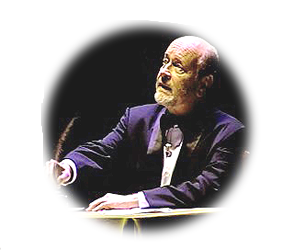
\includegraphics[width=3.5cm]{../misc/mastro}}\end{center}

\tableofcontents\newpage
 
\section{Referencia}%%%%%%%%%%%%%%%%%%REFERENCIA%%%%%%%%%%%%%%%%%%
\begin{tabular}{|l|l|p{5.4cm}|} \hline
\textbf{Algorítmo} & \textbf{Parámetros} &  \textbf{Función} \\  \hline
%swap & e1, e2 &  da vuelta e1,e2 & $1$\\\hline
sort, stable\_sort & f, l &  ordena el intervalo \\  \hline
%is\_sorted & f, l &  \textit{bool} si esta ordenado \\  \hline
nth\_element & f, nth, l & \textit{void} ordena el n-esimo, y \\ && particiona el resto \\  \hline
fill, fill\_n & f, l / n, elem & \textit{void} llena [f, l) o [f, \\ && f+n) con elem \\  \hline
lower\_bound, upper\_bound & f, l, elem & \textit{it} al primer / ultimo donde se \\ && puede insertar elem para que\\ && quede ordenada \\  \hline
binary\_search & f, l, elem & \textit{bool} esta elem en [f, l) \\  \hline
copy & f, l, resul & hace resul+$i$=f+$i$ $\forall i$ \\  \hline
find, find\_if, find\_first\_of & f, l, elem & \textit{it} encuentra i $\in$[f,l) tq. i$=$elem, \\ & / pred / f2, l2 & pred(i), i$\in$[f2,l2)\\\hline
count, count\_if & f, l, elem/pred & cuenta elem, pred(i)\\\hline
search & f, l, f2, l2 & busca [f2,l2) $\in$ [f,l)\\\hline
replace, replace\_if & f, l, old & cambia old / pred(i) por new \\ & / pred, new &\\\hline
reverse & f, l & da vuelta\\\hline
partition, stable\_partition & f, l, pred & pred(i) ad, !pred(i) atras\\\hline
%min, max & e1, e2 & men / may & $1$\\\hline
min\_element, max\_element & f, l, [comp] & \textit{it} min, max de [f,l]\\\hline
lexicographical\_compare & f1,l1,f2,l2 & \textit{bool} con [f1,l1]<[f2,l2]\\\hline
next/prev\_permutation & f,l & deja en [f,l) la perm sig, ant\\\hline
set\_intersection, & f1, l1, f2, l2, res & [res, $\ldots$) la op. de conj\\
set\_difference, set\_union, & & \\
set\_symmetric\_difference, & &\\\hline
push\_heap, pop\_heap, & f, l, e / e / & mete/saca e en heap [f,l), \\
make\_heap & & hace un heap de [f,l)\\\hline
is\_heap & f,l & \textit{bool} es [f,l) un heap\\\hline
accumulate & f,l,i,[op] & \textit{T} $=$ $\sum$/oper de [f,l)\\\hline
inner\_product & f1, l1, f2, i & \textit{T} $=$ i $+$ [f1, l1) . [f2, $\ldots$ )\\\hline
partial\_sum & f, l, r, [op] & r+i = $\sum$/oper de [f,f+i] $\forall i \in$[f,l)\\\hline
%power & e, i, op & \textit{T} = $e^{n}$\\\hline
\_\_builtin\_ffs& unsigned int & Pos. del primer 1 desde la derecha\\\hline
\_\_builtin\_clz & unsigned int & Cant. de ceros desde la izquierda.\\\hline
\_\_builtin\_ctz & unsigned int & Cant. de ceros desde la derecha.\\\hline
\_\_builtin\_popcount & unsigned int & Cant. de 1’s en x.\\\hline
\_\_builtin\_parity & unsigned int & 1 si x es par, 0 si es impar.\\\hline
\_\_builtin\_XXXXXXll & unsigned ll & = pero para long long's.\\\hline
\end{tabular}\newpage


\section{Estructuras}%%%%%%%%%%%%%%%%%%ESTRUCTURAS%%%%%%%%%%%%%%%%%%
\subsection{RMQ (static)}
\cppfile{../structures/rmq.static.cpp}
\subsection{RMQ (dynamic)}
\cppfile{structures/rmq.dynamic.cpp}
\subsection{RMQ (lazy)}
\cppfile{structures/rmq.lazy.cpp}
\subsection{RMQ (persistente)}
\cppfile{structures/rmq.persistent.cpp}
\subsection{Sliding window RMQ}
\cppfile{structures/sliding-window-rmq.cpp}
\subsection{Fenwick Tree}
\cppfile{structures/fenwick.cpp}
\subsection{Union Find}
\cppfile{structures/union.find.cpp}
\subsection{Disjoint Intervals}
\cppfile{structures/disjoint.intervals.cpp}
\subsection{RMQ (2D)}
\cppfile{structures/rmq.2d.cpp}
\subsection{Big Int}
\cppfile{structures/bigint.cpp}
\subsection{Hash}
\cppfile[22-66]{strings/hash_nico.cpp}
\subsection{Modnum}
\cppfile{structures/mod.cpp}
\subsection{Treap para set}
\cppfile[1-74]{structures/treap.cpp}
\subsection{Treap para arreglo}
\cppfile[1-73]{structures/treaparr.cpp}
\subsection{Convex Hull Trick}
\cppfile[4-56]{structures/convexhull.trick.cpp}
\subsection{Convex Hull Trick (Dynamic)}
\cppfile[17-56]{structures/convexhull.trick.dyn.cpp}
\subsection{Gain-Cost Set}
\cppfile[1-24]{structures/gain-cost.set.cpp}
\subsection{Set con índices}
\cppfile{structures/order.tree.cpp}


\section{Algoritmos}%%%%%%%%%%%%%%%%%%ALGORITMOS%%%%%%%%%%%%%%%%%%%%%%%%%%
\subsection{Longest Increasing Subsecuence}
\cppfile[1-31]{others/lis.cpp}
\subsection{Alpha-Beta prunning}
\cppfile{others/alphabeta.cpp}
\subsection{Mo's algorithm}
\cppfile{others/mosalgorithm.cpp}


\section{Strings}%%%%%%%%%%%%%%%%%%STRINGS%%%%%%%%%%%%%%%%%%%%%%%%%%
\subsection{Manacher}
\textbf{Definición: } permite calcular todas las substrings
de una string $s$ que son palíndromos de longitud impar (y par, ver 
\emph{observación}) . Para ello, mantiene un arreglo $len$ tal que $len[i]$ 
almacena la longitud del palíndromo impar maximal con centro en $i$. \\
\textbf{Explicación algoritmo: } muy similar al algoritmo para calcular
la \emph{función Z}. Mantiene el palíndromo que termina más a la derecha
entre todos los palíndromos ya detectados. Para calcular $len[i]$, utiliza
la información ya calculada si $i$ está dentro de $[l, r]$, y luego corre
el algoritmo trivial. \\
\textbf{Observación: } para calcular los palíndromos de longitud par, basta
con utilizar el mismo algoritmo con la cadena $s_0\#s_1\#...\#s_{n-1}$.
\cppfile{strings/manacher.cpp}
\subsection{KMP}
\cppfile{strings/kmp.cpp}
\subsection{Trie}
\cppfile{strings/trie.cpp}
%\subsection{Suffix Array (corto, nlog2n)}
%\cppfile[12-26]{string/suffix.array.short.cpp}
\subsection{Suffix Array (largo, nlogn)}
\cppfile[1-38]{strings/suffix.array.cpp}
\subsection{String Matching With Suffix Array}
\cppfile[38-59]{strings/suffix.array.cpp}
\subsection{LCP (Longest Common Prefix)}
\cppfile[61-75]{strings/suffix.array.cpp}
\subsection{Corasick}
\cppfile[1-36]{strings/corasick.cpp}
\subsection{Suffix Automaton}
\textbf{Definición}
Un suffix automaton $A$ es un autómata minimal que reconoce los sufijos de una 
cadena $s$.

\textbf{Conceptos importantes}
\begin{itemize}
    \item $A$ \emph{reconoce} a una cadena $s$ si comenzando desde el nodo inicial llegamos a un 
    terminal.

    \item Llamamos \emph{endpoints} de una cadena $u$ en $s$ a las posiciones $i$ tal que 
    $u = s_{i-|u|, i-1}$

    \item Dos substrings $u$ y $v$ de $s$ son \emph{equivalentes} si recorrer el autómata con $u$ 
    y con $v$ nos lleva al mismo nodo. Esto equivale a que los endpoints de $u$ y de
    $v$ en $s$ sean los mismos. 

    \item Los nodos del automáta corresponden a las \emph{clases de equivalencia} bajo la
    relación anterior.

    \item Si tomamos la \emph{cadena minimal} de una clase y removemos la primera letra,
    nos movemos al padre en el \emph{suffix tree} de $s'$. Esto se señaliza mediante \emph{suffix links}.
        
    \item Si tomamos la \emph{cadena maximal} de una clase y agregamos una letra al principio,
    nos movemos a otra clase de equivalencia, recorriendo un \emph{suffix link} en sentido inverso,
    es decir, nos movemos a los hijos en el suffix tree de $s'$.
\end{itemize}

\textbf{Problemas clásicos}
\begin{itemize}
    \item Determinar si $w$ es subcadena de $s$: simplemente correr el autómata.
    \item Determinar si $w$ es sufijo de $s$: correr el autómata y ver si caemos en un terminal.
    \item Contar cantidad de subcadenas distintas de $s$: esto es igual a la cantidad de
    caminos en el autómata y se calcula mediante una DP.
    \item Contar cantidad de apariciones de $w$ en $s$: correr autómata con $w$. Llamemos $u$
    al nodo en el que terminamos, la cantidad de apariciones es la cantidad de caminos 
    en $A$ que comienzan en $u$ y llegan a un terminal.
    \item Encontrar dónde aparece $w$ por primera vez en $s$: correr autómata con $w$. Llamemos $u$
    al nodo en el que terminamos, esto equivale a calcular el camino más largo del autómata 
    a partir del nodo $u$.
    \item Encontrar las posiciones de todas las apariciones de $w$ en $s$: agregar '\$' a $s$,
    encontrar el nodo $u$ en el que finaliza $w$, armar el \emph{suffix tree}, encontrar
    todas las hojas en el subárbol con raíz en $u$, cada hoja corresponde a un prefijo
    y por lo tanto a una aparición.
\end{itemize}
\cppfile[1-46]{strings/suffix.automaton.cpp}
\subsection{Z Function}
\textbf{Definición}
La función Z para una string $s$ de longitud $n$ es un arreglo $a$ de la misma longitud
tal que $a[i]$ es la \emph{máxima cantidad de caracteres} comenzando desde la posición $i$
que coinciden con los primeros caracteres de $s$. Es decir, es el \emph{máximo prefijo común}.

\textbf{Observación}
$z[0]$ no está bien definido, pero se asume igual a $0$.

\textbf{Algoritmo}
La idea es mantener el máximo \emph{match} (es decir, el segmento $[l, r]$ con
máximo $r$ tal que se sabe que $s[0..r-l] = s[l..r]$). 

Siendo $i$ el índice actual (del que queremos calcular la función Z), el algoritmo 
se divide en dos casos:
\begin{itemize}
    \item $i > r$: la posición está fuera de lo que hemos procesado. Se corre el
    \emph{algoritmo trivial}.
    \item $i <= r$: la posición está dentro del \emph{match actual}, por lo que
    se puede utilizar como aproximación inicial $z[i] = min(r - i + 1, z[i-l])$,
    y luego correr el \emph{algoritmo trivial}.
\end{itemize}

\textbf{Problemas clásicos}
\begin{itemize}
    \item Buscar una subcadena: concatenamos $p$ con $t$ (utilizando un separador).
    Hay una aparición si la función Z matcheó tantos caracteres como la longitud
    de $p$.
\end{itemize}
\cppfile{strings/zfunction.cpp}
\subsection{Palindrome}
\cppfile{strings/palindrome.cpp}

\section{Geometría}%%%%%%%%%%%%%%%%%%geometria%%%%%%%%%%%%%%%%%%%%%%
\subsection{Punto}
\cppfile[2-33]{geometry/pto.cpp}
\subsection{Orden radial de puntos}
\cppfile{geometry/orden.radial.cpp}
\subsection{Line}
\cppfile{geometry/line.cpp}
\subsection{Segment}
\cppfile{geometry/segm.cpp}
\subsection{Rectangle}
\cppfile{geometry/rect.cpp}
\subsection{Polygon Area}
\cppfile{geometry/area.cpp}
\subsection{Circle}
\cppfile{geometry/circle.cpp}
\subsection{Point in Poly}
\cppfile{geometry/point.in.poly.cpp}
\subsection{Point in Convex Poly log(n)}
\cppfile{geometry/point.in.convex.poly.cpp}
\subsection{Convex Check CHECK}
\cppfile{geometry/convex.check.cpp}
\subsection{Convex Hull}
\cppfile{geometry/convex.hull.cpp}
\subsection{Cut Polygon}
\cppfile{geometry/cut.polygon.cpp}
\subsection{Bresenham}
\cppfile{geometry/bresenham.cpp}
\subsection{Rotate Matrix}
\cppfile{geometry/rotate.cpp}
\subsection{Interseccion de Circulos en n3log(n)}
\cppfile{geometry/int.circs.cpp}

\subsection{Cayley-Menger}
{
Permite calcular el volumen de un simplex (triángulo en k dimensiones) mediante el cálculo de una determinante.
\cppfile[65-82]{geometry/cayley.cpp}
}

\subsection{Heron's formula}
{
It states that the area of a triangle whose sides have lengths a, b, and c is

\( {\displaystyle A={\sqrt {s(s-a)(s-b)(s-c)}}} \),
where s is the semiperimeter of the triangle; that is,

\( {\displaystyle s={\frac {a+b+c}{2}}} \).
}

\section{DP Opt}
Observaciones:

$A[i][j]$ el menor $k$ que logra la solución óptima. En Knuth y D\&C la idea es aprovechar los rangos
determinados por este arreglo.

\subsection{Knuth}
{
    \textbf{Problema de ejemplo:} dado un palito de longitud $l$, con $n$ puntos en los que se puede cortar,
    determinar el costo mínimo para partir el palito en $n+1$ palitos unitarios (la DP se puede adaptar a $k$ 
    agregando un parámetro extra), donde hay un costo fijo por partir el rango $i, j$ que \emph{cumple la 
    condición suficiente}. Una función de costos que cumple es la distancia entre los extremos $j-i$. 
    El problema clásico de esta pinta es el del ABB óptimo.

    \textbf{Recurrencia original:} $dp[i][j] = min_{i < k < j} {dp[i][k] + dp[k][j]} + C[i][j]$

    \textbf{Condición suficiente:} $A[i, j - 1] \leq  A[i, j] \leq A[i + 1, j]$

    Es decir, si saco un elemento a derecha el óptimo se mueve a izquierda o se mantiene, y 
    análogo si saco un elemento a izquierda.

    \textbf{Complejidad original:} $O(n^3)$

    \textbf{Complejidad optimizada:} $O(n^2)$

    \textbf{Solución:} iteramos por el tamaño $len$ del subarreglo (creciente), y para cada extremo izquierdo $l$,
    determinamos el extremo derecho $r=l+len$ e iteramos por los $k$ entre $A[l][r-1]$ y $A[l+1][r]$, actualizando la
    solución del estado actual.
}
\subsection{Chull}
{
    \textbf{Problema de ejemplo:} 

    \textbf{Recurrencia original:}

    \textbf{Condición suficiente:} 

    \textbf{Complejidad original:} 

    \textbf{Complejidad optimizada:} 

    \textbf{Solución:} 
}
\subsection{Divide \& Conquer}
{
    \textbf{Problema de ejemplo:} dado un arreglo de $n$ números con valores $a_1, a_1, \dots, a_n$, dividirlo
    en $k$ subarreglos, tal que la suma de los cuadrados del peso total de cada subarreglo es mínimo.

    \textbf{Recurrencia original:} $dp[i][j] = min_{k < j}{dp[i - 1][k] + C[k][j]}$ 

    \textbf{Condición suficiente:} $ A[i][j] \leq A[i][j + 1] $ o (normalmente más fácil de probar) 
    $ C[a][d] + C[b][c] \geq C[a][c] + C[b][d]$, con $a < b < c < d. $.

    La segunda condición suficiente es la intuición de que no conviene que los intervalos se crucen.

    \textbf{Complejidad original:} $O(kn^2)$

    \textbf{Complejidad optimizada:} $O(kn\log(n))$

    \textbf{Solución:} la idea es, para un $i$ determinado, partir el rango $[j_{left}, j_{right})$ al que pertenecen 
    los $j$ que queremos calcular a la mitad, determinar el óptimo y utilizarlo como límite para calcular los demás.
    Para implementar esto de forma sencilla, se suele utilizar la función recursiva $dp(i, j_{left}, j_{right}, opt_{left}, opt_{right})$
    que se encarga de, una vez fijado el punto medio $m$ del rango $[j_{left}, j_{right})$ iterar por los $k$ en $[j_{left}, j_{right})$ 
    para determinar el óptimo $opt$ para $m$, y continuar calculando $dp(i, j_{left}, m, opt_{left}, opt)$ y 
    $dp(i, m, j_{right}, opt, opt_{right})$.
}


\section{Matemática}%%%%%%%%%%%%%%%%%%MATH%%%%%%%%%%%%%%%%%%%%%%%%%%%%%%%%
\subsection{Teoría de números}
{
\subsubsection{Teorema de Wilson}
{
\(\displaystyle (p-1)! \equiv -1 \;(\bmod\; p) \)
Siendo $p$ primo.
}
\subsubsection{Pequeño teorema de Fermat}
{
\(\displaystyle a^p \equiv a \;(\bmod\; p) \)
Siendo $p$ primo.
}
\subsubsection{Teorema de Euler}
{
\(\displaystyle a^{\varphi(n)} \equiv 1 \;(\bmod\; n) \)
}
}
\subsection{Combinatoria}
{
\subsubsection{Burnside's lemma}
{
Sea $G$ un grupo que actúa en un conjunto $X$. Para cada $g$ en $G$, sea $X^{g}$ el conjunto de elementos
en $X$ que son invariantes respecto a $g$, entonces el número de órbitas $|X/G|$ es:
\[ |X/G|={\frac {1}{|G|}}\sum _{{g\in G}}|X^{g}|.\]
Por ejemplo, si el grupo $G$ consiste de las operaciones de rotación, el conjunto $X$ son los posibles coloreos de un tablero, 
entonces el número de órbitas $|X/G|$ es el número de posibles coloreos de un tablero salvo rotaciones.
}

\subsubsection{Combinatorios}
{
\(\displaystyle \binom{n}{k} = \frac{n!}{k!(n-k)!} \)
\cppfile[9-13]{math/combinatorics.cpp}
}

\subsubsection{Lucas Theorem}
{
    \(\displaystyle {\binom {m}{n}}\equiv \prod_{i=0}^{k}{\binom {m{i}}{n_{i}}}{\pmod{p}}\)

where \({\displaystyle m=m_{k}p^{k}+m_{k-1}p^{k-1}+\cdots +m_{1}p+m_{0},}\)

and \({\displaystyle n=n_{k}p^{k}+n_{k-1}p^{k-1}+\cdots +n_{1}p+n_{0}}\)

\({\displaystyle {\tbinom {m}{n}}=0}\) if \(m < n\).


\cppfile[22-26]{math/combinatorics.cpp}
}
\subsubsection{Stirling}
{
\(\displaystyle \left\{{n \atop k}\right\} = \) cantidad de formas de particionar un conjunto de \(n\) elementos en \(m\) subconjuntos no vacíos.

\(\displaystyle \left\{{n+1\atop k}\right\} = k \left\{{ n \atop k }\right\} + \left\{{n\atop k-1}\right\}\)

for \(k > 0\) with initial conditions

\({\displaystyle \left\{{0 \atop 0}\right\}=1\quad {\mbox{ and }}\quad \left\{{n \atop 0}\right\}=\left\{{0 \atop n}\right\}=0}\)
for \(n > 0\).


\cppfile[1-7]{math/combinatorics.cpp}
}
\subsubsection{Bell}
{
\( {\displaystyle B_{n}=} \) cantidad de formas de particionar un conjunto de \(n\) elementos en subconjuntos no vacíos.

\( {\displaystyle B_0= B_1 = 1} \)

\( {\displaystyle B_{n+1}=\sum_{k=0}^{n} \binom{n}{k} B_k.} \) 

\( {\displaystyle B_{n}=\sum _{k=0}^{n}\left\{{n \atop k}\right\}.} \) 


\cppfile[15-20]{math/combinatorics.cpp}
} 
\subsubsection{Eulerian}
{
\( {\displaystyle A_{n, m}=} \) cantidad de permutaciones de 1 a n con m ascensos (m elementos mayores que el anterior).

\( {\displaystyle A(n,m)=(n-m)A(n-1,m-1)+(m+1)A(n-1,m).} \)
}
\subsubsection{Catalan}
{
\( {\displaystyle C_{n}=} \) cantidad de árboles binarios de n+1 hojas, en los que cada nodo tiene cero o dos hijos.

\({\displaystyle C_{n}={2n \choose n}-{2n \choose n-1}\quad {\mbox{ con }}n\geq 1.} \)

\( {\displaystyle C_{0}=1\quad {\mbox{y}}\quad C_{n+1}=\sum _{i=0}^{n}C_{i}\,C_{n-i}\quad {\mbox{con }}n\geq 0.} \)
}

}

\subsection{Sumatorias conocidas}
{
$\sum_{i=0}^n\binom{n}{i}=2^n$

$\sum_{i=0}^n i\binom{n}{i}=n*2^{n-1}$

$\sum_{i=m}^n i = \frac{n(n+1)}{2} - \frac{m(m-1)}{2} = \frac{(n+1-m)(n+m)}{2}$

$\sum_{i=0}^n i = \sum_{i=1}^n i = \frac{n(n+1)}{2}$

$\sum_{i=0}^n i^2 = \frac{n(n+1)(2n+1)}{6} = \frac{n^3}{3} + \frac{n^2}{2} + \frac{n}{6}$

$\sum_{i=0}^n i(i-1) = \frac{8}{6}(\frac{n}{2})(\frac{n}{2}+1)(n+1)$ (doubles) $\rightarrow$ Sino ver caso impar y par

$\sum_{i=0}^n i^3 = \left(\frac{n(n+1)}{2}\right)^2 = \frac{n^4}{4} + \frac{n^3}{2} + \frac{n^2}{4} = \left[\sum_{i=1}^n i\right]^2$

$\sum_{i=0}^n i^4 = \frac{n(n+1)(2n+1)(3n^2+3n-1)}{30} = \frac{n^5}{5} + \frac{n^4}{2} + \frac{n^3}{3} - \frac{n}{30}$

$\sum_{i=0}^n i^p = \frac{(n+1)^{p+1}}{p+1} + \sum_{k=1}^p\frac{B_k}{p-k+1}{p\choose k}(n+1)^{p-k+1}$

}

\subsection{Ec. Característica}
$a_0T(n)+a_1T(n-1)+...+a_kT(n-k)=0$

$p(x)=a_0 x^k + a_1 x^{k-1} + ... + a_k$

Sean $r_1,r_2,...,r_q$ las raíces distintas, de mult. $m_1, m_2, ..., m_q$

$T(n)=\sum_{i=1}^q{\sum_{j=0}^{m_i - 1}c_{ij} n^j r_i^n}$

Las constantes $c_{ij}$ se determinan por los casos base.
\subsection{Aritmetica Modular}
\cppfile{math/modular_arithmetic.cpp}
\subsection{Exp. de Numeros Mod.}
\cppfile{math/exp.mod.cpp}
\subsection{Exp. de Matrices y Fibonacci en log(n)}
\cppfile{math/exp.mat.cpp}
\subsection{Matrices y determinante $O(n^3)$}
\cppfile[1-36]{math/determinante.cpp}
\subsection{Primes and factorization}
\cppfile{math/factorize.cpp}
\subsection{Euler's Phi}
\cppfile[1-23]{math/phi_euler.cpp}
\subsection{Criba}
\cppfile[1-17]{math/criba.cpp}
\subsection{Funciones de primos}
Sea $n=\prod{p_i^{k_i}}$, fact(n) genera un map donde a cada $p_i$ le asocia su $k_i$
\cppfile{math/func.primos.cpp}
\subsection{Phollard's Rho - Miller-Rabin}
\cppfile[16-78]{math/phollards.rho.cpp}
\subsection{GCD}
\cppfile[1-2]{math/GCD-LCM.cpp}
\subsection{LCM}
\cppfile[3]{math/GCD-LCM.cpp}
\subsection{Euclides extendido}
Dados $a$ y $b$, encuentra $x$ e $y$ tales que $a*x + b*y = gcd(a, b)$.
\cppfile{math/extended.euclid.cpp}
\subsection{Inversos}
\cppfile{math/inversos.cpp}
\subsection{Ecuaciones diofánticas}
Basado en Euclides extendido. Dados $a$, $b$, y $r$ obtiene $x$ e $y$ tales que $a*x + b*y = r$, suponiendo que $gcd(a,b) | r$. Las soluciones son de la forma $(x, y) = (x_1 - b/gcd(a,b) * k_1, x_2 + a/gcd(a,b) * k_2)$ donde $x_1$ y $x_2$ son las soluciones particulares que obtuvo Euclides.
\cppfile{math/diophantine.cpp}
\subsection{Teorema Chino del Resto}
Dadas $k$ ecuaciones de la forma $a_i*x \equiv a_i \pmod {n_i}$, encuentra $x$ tal que es solución. Existe una única solución módulo $lcm(n_i)$.
\cppfile{math/chinese.cpp}
\subsection{Simpson}
\cppfile{math/simpson.cpp}
\subsection{Fraction}
\cppfile{math/frac.cpp}
\subsection{Polinomio, Ruffini e interpolación de Lagrange}
\textbf{Interpolación de Lagrange}: dados $n+1$ pares $(x_i, y_i)$  permite encontrar el polinomio de grado $n$ tal que $f(x_i) = y_i$. 

\textbf{Explicación}: computa $P(x) = y_1*f_1(x) + y_2*f_2(x) + \ldots + y_{n+1}*f_{n+1}(x)$ donde $f_i(x) = \frac{g_i(x)}{g_i(x_i)}$, $g_i(x) = \frac{h(x)}{x - x_i}$ y $h(x) = (x-x_1)*(x-x_2)*\ldots*(x-x_{n+1})$.
Usa Ruffini para la división de polinomios.

Trucazo para computar en \(O(n)\): \(x_{i + 1} - x_i = x_{j + 1} - x_j\) para todo \(i, j < n\).

\textbf{Ejemplo de problema}: tenés que calcular una respuesta que depende de un n y parece ser polinomial, conseguís un par de puntos e 
intentás armar el polinomio (usando el algoritmo online u offline).

\cppfile{math/polinomio.cpp}
\subsection{Ec. Lineales}
\cppfile[29-62]{math/eclineales.cpp}
\subsection{FFT y NTT}

\textbf{Base teórica} \\
Dado el espacio lineal con producto interno (definido como una integral loca) 
$E$, de funciones continuas definidas por partes $f \colon [-\pi, \pi] \rightarrow \mathbb{C}$, 
un \textbf{sistema ortonormal cerrado infinito} es $\{1/\sqrt(2), \sin(x), \cos(x), \sin(2x), 
\cos(2x), ...\}$.  Por lo tanto, cualquier funcion $f \in E$ puede ser representada por 
$\sum_{n=1}^{\infty} \langle f,\ e_n \rangle e_n$. Esta combinación lineal (utilizando
la sumatoria y el sistema ya definidos), es la \textbf{serie de Fourier}. \\ 
También se puede definir la \textbf{serie compleja de Fourier} mediante el
sistema $\{1, e^{ix}, e^{-ix}, e^{i2x}, e^{-i2x}, ...\}$. \\
Una \textbf{transformada de Fourier} permite trabajar con funciones que no están
restringidas al intervalo $[-\pi, \pi]$. La principal diferencia es que el sistema
ortonormal pasa de ser discreto a continuo. \\
Sin embargo, existe una versión discreta de la transformada, la \textbf{transformada 
discreta de Fourier} (DFT). \\
Una de las propiedades importantes de la transformada es que la \textbf{convolución} 
de funciones sin transformar se traduce en multiplicar las transformadas. \\
\textbf{FFT}, el algoritmo para calcular rápidamente la DFT, se basa en que
dado un polinomio $A(x)$, $A(x) = A_0(x^2) + x*A_1(x^2)$, donde $A_0(x)$ y $A_1(x)$ 
son los polinomios que se forman al tomar los términos pares e impares respectivamente. \\
\textbf{NTT} es un algoritmo más lento pero más preciso para calcular la DFT,
ya que trabaja con enteros módulo un primo $p$.

\cppfile{math/fft_y_ntt.cpp}

\subsection{Tablas y cotas (Primos, Divisores, Factoriales, etc)}
%\subsubsection{
\paragraph{Factoriales} \ \\
\begin{tabular}{l|l}
0! =	1             & 11! = 39.916.800  \\
1! =	1             & 12! =	479.001.600	($\in \mathtt{int}$)\\
2! =	2             & 13! =	6.227.020.800	\\
3! =	6             & 14! =	87.178.291.200	\\
4! =	24            & 15! =	1.307.674.368.000	\\
5! =	120   			  & 16! =	20.922.789.888.000	\\
6! =	720           & 17! =	355.687.428.096.000	\\
7! =	5.040	        & 18! =	6.402.373.705.728.000	\\
8! =	40.320	      & 19! =	121.645.100.408.832.000	\\
9! =	362.880       & 20! =	2.432.902.008.176.640.000	($\in \mathtt{tint}$) \\
10! =	3.628.800     & 21! =	51.090.942.171.709.400.000
\end{tabular}
 
max signed tint = 9.223.372.036.854.775.807 \\
max unsigned tint = 18.446.744.073.709.551.615
%\subsubsection{
\paragraph{Primos} \ \\
2 3 5 7 11 13 17 19 23 29
31 37 41 43 47 53 59 61 67 71
73 79 83 89 97 101 103 107 109 113
127 131 137 139 149 151 157 163 167 173
179 181 191 193 197 199 211 223 227 229
233 239 241 251 257 263 269 271 277 281
283 293 307 311 313 317 331 337 347 349
353 359 367 373 379 383 389 397 401 409
419 421 431 433 439 443 449 457 461 463
467 479 487 491 499 503 509 521 523 541
547 557 563 569 571 577 587 593 599 601
607 613 617 619 631 641 643 647 653 659
661 673 677 683 691 701 709 719 727 733
739 743 751 757 761 769 773 787 797 809
811 821 823 827 829 839 853 857 859 863
877 881 883 887 907 911 919 929 937 941
947 953 967 971 977 983 991 997 1009 1013
1019 1021 1031 1033 1039 1049 1051 1061 1063 1069
1087 1091 1093 1097 1103 1109 1117 1123 1129 1151
1153 1163 1171 1181 1187 1193 1201 1213 1217 1223
1229 1231 1237 1249 1259 1277 1279 1283 1289 1291
1297 1301 1303 1307 1319 1321 1327 1361 1367 1373
1381 1399 1409 1423 1427 1429 1433 1439 1447 1451
1453 1459 1471 1481 1483 1487 1489 1493 1499 1511
1523 1531 1543 1549 1553 1559 1567 1571 1579 1583
1597 1601 1607 1609 1613 1619 1621 1627 1637 1657
1663 1667 1669 1693 1697 1699 1709 1721 1723 1733
1741 1747 1753 1759 1777 1783 1787 1789 1801 1811
1823 1831 1847 1861 1867 1871 1873 1877 1879 1889
1901 1907 1913 1931 1933 1949 1951 1973 1979 1987
1993 1997 1999 2003 2011 2017 2027 2029 2039 2053
2063 2069 2081
 
%2083 2087 2089 2099 2111 2113 2129
%2131 2137 2141 2143 2153 2161 2179 2203 2207 2213
%2221 2237 2239 2243 2251 2267 2269 2273 2281 2287
%2293 2297 2309 2311 2333 2339 2341 2347 2351 2357
%2371 2377 2381 2383 2389 2393 2399 2411 2417 2423
%2437 2441 2447 2459 2467 2473 2477 2503 2521 2531
%2539 2543 2549 2551 2557 2579 2591 2593 2609 2617
%2621 2633 2647 2657 2659 2663 2671 2677 2683 2687
%2689 2693 2699 2707 2711 2713 2719 2729 2731 2741
%2749 2753 2767 2777 2789 2791 2797 2801 2803 2819
%2833 2837 2843 2851 2857 2861 2879 2887 2897 2903
%2909 2917 2927 2939 2953 2957 2963 2969 2971 2999
%3001 3011 3019 3023 3037 3041 3049 3061 3067 3079
%3083 3089 3109 3119 3121 3137 3163 3167 3169 3181
%3187 3191 3203 3209 3217 3221 3229 3251 3253 3257
%3259 3271 3299 3301 3307 3313 3319 3323 3329 3331
%3343 3347 3359 3361 3371 3373 3389 3391 3407 3413
%3433 3449 3457 3461 3463 3467 3469 3491 3499 3511
%3517 3527 3529 3533 3539 3541 3547 3557 3559 3571\\
\paragraph{Primos cercanos a $10^n$}\ \\
9941 9949 9967 9973 10007 10009 10037 10039 10061 10067 10069 10079\\
99961 99971 99989 99991 100003 100019 100043 100049 100057 100069\\
999959 999961 999979 999983 1000003 1000033 1000037 1000039\\
9999943 9999971 9999973 9999991 10000019 10000079 10000103 10000121\\
99999941 99999959 99999971 99999989 100000007 100000037 100000039 100000049\\
999999893 999999929 999999937 1000000007 1000000009 1000000021 1000000033
 
\paragraph{Cantidad de primos menores que $10^n$}\ \\
$\pi(10^1)$ = 4 ;
$\pi(10^2)$ = 25 ;
$\pi(10^3)$ = 168 ;
$\pi(10^4)$ = 1229 ;
$\pi(10^5)$ = 9592 \\
$\pi(10^6)$ = 78.498 ;
$\pi(10^7)$ = 664.579 ;
$\pi(10^8)$ = 5.761.455 ;
$\pi(10^9)$ = 50.847.534 \\
$\pi(10^{10})$ = 455.052,511 ;
$\pi(10^{11})$ = 4.118.054.813 ;
$\pi(10^{12})$ = 37.607.912.018 \\
\textbf{Observación:} Una buena aproximación es $x/ln(x)$.
%
% Fuente: http://primes.utm.edu/howmany.shtml#table
%
%
%\subsubsection{Divisores}
\paragraph{Divisores} \ \\
Cantidad de divisores ($\sigma_0$) para \emph{algunos} $n / \neg\exists n'<n, \sigma_0(n') \geqslant \sigma_0(n)$ \\
\textbf{Referencias:} $\sigma_0(10^9) = 1344$ y $\sigma_0(10^{18}) = 103680$ \\
$\sigma_0(60)$ = 12 ; $\sigma_0(120)$ = 16 ; $\sigma_0(180)$ = 18 ; $\sigma_0(240)$ = 20 ; $\sigma_0(360)$ = 24 \\
$\sigma_0(720)$ = 30 ; $\sigma_0(840)$ = 32 ; $\sigma_0(1260)$ = 36 ; $\sigma_0(1680)$ = 40 ; $\sigma_0(10080)$ = 72 \\ $\sigma_0(15120)$ = 80 ; $\sigma_0(50400)$ = 108 ; $\sigma_0(83160)$ = 128 ; $\sigma_0(110880)$ = 144 \\
$\sigma_0(498960)$ = 200 ; $\sigma_0(554400)$ = 216 ; $\sigma_0(1081080)$ = 256 ; $\sigma_0(1441440)$ = 288  $\sigma_0(4324320)$ = 384 ; $\sigma_0(8648640)$ = 448 \\
\textbf{Observación:} Una buena aproximación es $x^{1/3}$. \\ \\
%
Suma de divisores ($\sigma_1$) para \emph{algunos} $n / \neg\exists n'<n, \sigma_1(n') \geqslant \sigma_1(n)$ \\
$\sigma_1(96)$ = 252 ; $\sigma_1(108)$ = 280 ; $\sigma_1(120)$ = 360 ; $\sigma_1(144)$ = 403 ; $\sigma_1(168)$ = 480 \\
$\sigma_1(960)$ = 3048 ; $\sigma_1(1008)$ = 3224 ; $\sigma_1(1080)$ = 3600 ; $\sigma_1(1200)$ = 3844 \\
$\sigma_1(4620)$ = 16128 ; $\sigma_1(4680)$ = 16380 ; $\sigma_1(5040)$ = 19344 ; $\sigma_1(5760)$ = 19890 \\
$\sigma_1(8820)$ = 31122 ; $\sigma_1(9240)$ = 34560 ; $\sigma_1(10080)$ = 39312 ; $\sigma_1(10920)$ = 40320 \\
$\sigma_1(32760)$ = 131040 ; $\sigma_1(35280)$ = 137826 ; $\sigma_1(36960)$ = 145152 ; $\sigma_1(37800)$ = 148800 \\
$\sigma_1(60480)$ = 243840 ; $\sigma_1(64680)$ = 246240 ; $\sigma_1(65520)$ = 270816 ; $\sigma_1(70560)$ = 280098 \\
$\sigma_1(95760)$ = 386880 ; $\sigma_1(98280)$ = 403200 ; $\sigma_1(100800)$ = 409448  \\
$\sigma_1(491400)$ = 2083200 ; $\sigma_1(498960)$ = 2160576 ; $\sigma_1(514080)$ = 2177280 \\
$\sigma_1(982800)$ = 4305280 ; $\sigma_1(997920)$ = 4390848 ; $\sigma_1(1048320)$ = 4464096 \\
$\sigma_1(4979520)$ = 22189440 ; $\sigma_1(4989600)$ = 22686048 ; $\sigma_1(5045040)$ = 23154768 \\
$\sigma_1(9896040)$ = 44323200 ; $\sigma_1(9959040)$ = 44553600 ; $\sigma_1(9979200)$ = 45732192
%
%


\section{Grafos}%%%%%%%%%%%%%%%%%%GRAFOS%%%%%%%%%%%%%%%%%%%%%%%%%%%%
\subsection{Teoremas y fórmulas}
{
\subsubsection{Teorema de Pick}
{
$A=I+\frac{B}{2}-1$

Donde \(A\) es el área, \(I\) es la cantidad de puntos interiores, y \(B\) la cantidad de puntos en el borde.
}

\subsubsection{Formula de Euler}
{
$v-e+f=k+1$

Donde \(v\) es la cantidad de vértices, \(e\) la cantidad de arcos, \(f\) la cantidad de caras y \(k\) la cantidad de componentes conexas.
}
}
\subsection{Dijkstra}
\cppfile{graphs/dijkstra.cpp}
\subsection{Bellman-Ford}
\cppfile{graphs/bellman.ford.cpp}
\subsection{Floyd-Warshall}
\cppfile{graphs/floyd.warshall.cpp}
\subsection{Kruskal}
\cppfile[27-41]{graphs/kruskal.cpp}
\subsection{Prim}
\cppfile[23-40]{graphs/prim.cpp}
\subsection{2-SAT + Tarjan SCC}
\cppfile{graphs/2sat.cpp}
\subsection{Kosaraju}
\cppfile[23-72]{graphs/kosaraju.cpp}
\subsection{Articulation Points}
\cppfile{graphs/articulaciones.cpp}
\subsection{Comp. Biconexas y Puentes}
\cppfile{graphs/biconexas.bridge.cpp}
\subsection{LCA + Climb}
\cppfile{graphs/lca.climb.cpp}
\subsection{Heavy Light Decomposition}
\cppfile{graphs/heavylight.cpp}
\subsection{Centroid Decomposition}
\cppfile[3-20]{graphs/centroid.cpp}
\subsection{Euler Cycle}
\cppfile{graphs/euler.cpp}
\subsection{Diametro árbol}
\cppfile{graphs/diametro.cpp}
\subsection{Chu-liu}
\cppfile{graphs/chuliu.cpp}
\subsection{Hungarian}
\cppfile[5-59]{graphs/hungarian.cpp}
\subsection{Dynamic Conectivity}
\cppfile[17-78]{graphs/dynamic.conectivity.cpp}


\section{Flujo}%%%%%%%%%%%%%%%%%%FLOW%%%%%%%%%%%%%%%%%%%%%%%%%%%%
\subsection{Dinic}
\cppfile{flow/dinic.cpp}
\subsection{Konig}
\cppfile[98-122]{flow/konig.cpp}
\subsection{Edmonds Karp's}
\cppfile{flow/edmonds.karp.cpp}
\subsection{Min-cost Max-flow}
\cppfile[16-66]{flow/min.cost.max.flow.cpp}


\section{Template}%%%%%%%%%%%%%%%%%%TEMPLATE%%%%%%%%%%%%%%%%
\cppfile{misc/template.cpp}

\section{Template hash}
\cppfile{misc/hash.txt}

\section{vimrc}
\cppfile{misc/vimrc.cpp}

\section{misc}
\cppfile{misc/truquillos.cpp}


\section{Ayudamemoria}%%%%%%%%%%%%%%%%%%AYUDAMEMORIA%%%%%%%%%%%%%%%%
\subsection*{Cant. decimales} 	
\begin{code}
#include <iomanip>
cout << setprecision(2) << fixed;
\end{code}
\subsection*{Rellenar con espacios(para justificar)}
\begin{code}
#include <iomanip>
cout << setfill(' ') << setw(3) << 2 << endl;
\end{code}
\subsection*{Comparación de Doubles}
\begin{code}
const double EPS = 1e-9;
x == y	<=> fabs(x-y) < EPS
x >  y	<=> x > y + EPS
x >= y	<=> x > y - EPS
\end{code}
\subsection*{Limites}
\begin{code}
#include <limits>
numeric_limits<T>
	::max()
	::min()
	::epsilon()
\end{code}
\subsection*{Muahaha}
\begin{code}
#include <signal.h>
void divzero(int p){
	while(true);}
void segm(int p){
	exit(0);}
//in main
signal(SIGFPE, divzero);
signal(SIGSEGV, segm);
\end{code}
\subsection*{Mejorar velocidad 2}
\begin{code}
//Solo para enteros positivos
inline void Scanf(int& a){
	char c = 0;
	while(c<33) c = getc(stdin);
	a = 0;
	while(c>33)	a = a*10 + c - '0', c = getc(stdin);
}
\end{code}
\subsection*{Leer del teclado}
\begin{code}
freopen("/dev/tty", "a", stdin);
\end{code}
\subsection*{Iterar subconjunto}
\begin{code}
for(int sbm=bm; sbm; sbm=(sbm-1)&bm)
\end{code}
\subsection*{File setup}
\begin{code}
// tambien se pueden usar comas: {a, x, m, l}
touch {a..l}.in; tee {a..l}.cpp < template.cpp
\end{code}
\subsection*{Releer String}
\begin{code}
string s; int n;
getline(cin, s);
stringstream leer(s);
while(leer >> n){
	// do something ...
}
\end{code}
\end{document}
